\documentclass{article}
\usepackage{graphicx, amsmath, amssymb, mathtools, float, fancyhdr, halloweenmath}

\graphicspath{{Images/}}

\setlength{\oddsidemargin}{0in}
\setlength{\textwidth}{6.5in}
\setlength{\topmargin}{-.55in}
\setlength{\textheight}{9in}
\pagestyle{fancy}

\fancyfoot{}
\fancyhead[R]{$\mathbat$ \thepage \hspace{0.07cm} $\mathbat$}
\fancyhead[L]{$\mathbat$ MATH 5430 $\mathbat$}



\begin{document}
\begin{center}
    {\Huge Homework 4}
    \vspace{0.5 cm}

    {\large Michael Nameika}
\end{center}


\section*{2D Linear Systems}
\begin{itemize}
    \item[1.] Consider the initial value problem $\dot{\mathbf{x}} = A\mathbf{x}(t)$, $\mathbf{x}(0) = \mathbf{x}_0$ for the following matrices. Characterize the stability of these systems. What type is it? Is it stable or unstable? Also, make a sketch of the system near the critical point. Note: these are the same systems you solved in Homework 3.
    \begin{itemize}
        \item[(a)] $A = \begin{pmatrix}
            1 & -2\\
            -2 & 1
        \end{pmatrix}$
        \newline\newline
        Notice that the origin, $\mathbf{x} = \mathbf{0}$ is the critical point of the system. (As will be the case for parts (b) and (c).) From Homework 3, we have $\lambda_1 = 3$, $\lambda_2 = -1$ with associated eigenvectors
        \[v_1 = \begin{pmatrix}
            -1\\
            1
        \end{pmatrix}, \hspace{0.3cm} v_2 = \begin{pmatrix}
            1\\
            1
        \end{pmatrix}.\]
        Since $\lambda_1 > 0$, $\lambda_2 < 0$, we have that the origin is a saddle. 
        \newline
        Additionally, for an initial condition on the line spanned by $v_1$, since $\lambda_1 > 0$, the solution will be repulsed away from the origin. However, for an initial condition on the line spanned by $v_2$, since $\lambda_2 < 0$, the solution will be attracted to the origin. Off these lines, the solution will be ``attracted" to the origin and then repulsed as it nears, as we can see in the following figure (the hand drawn figures got rotated for some reason, apologies):
        \begin{center}
            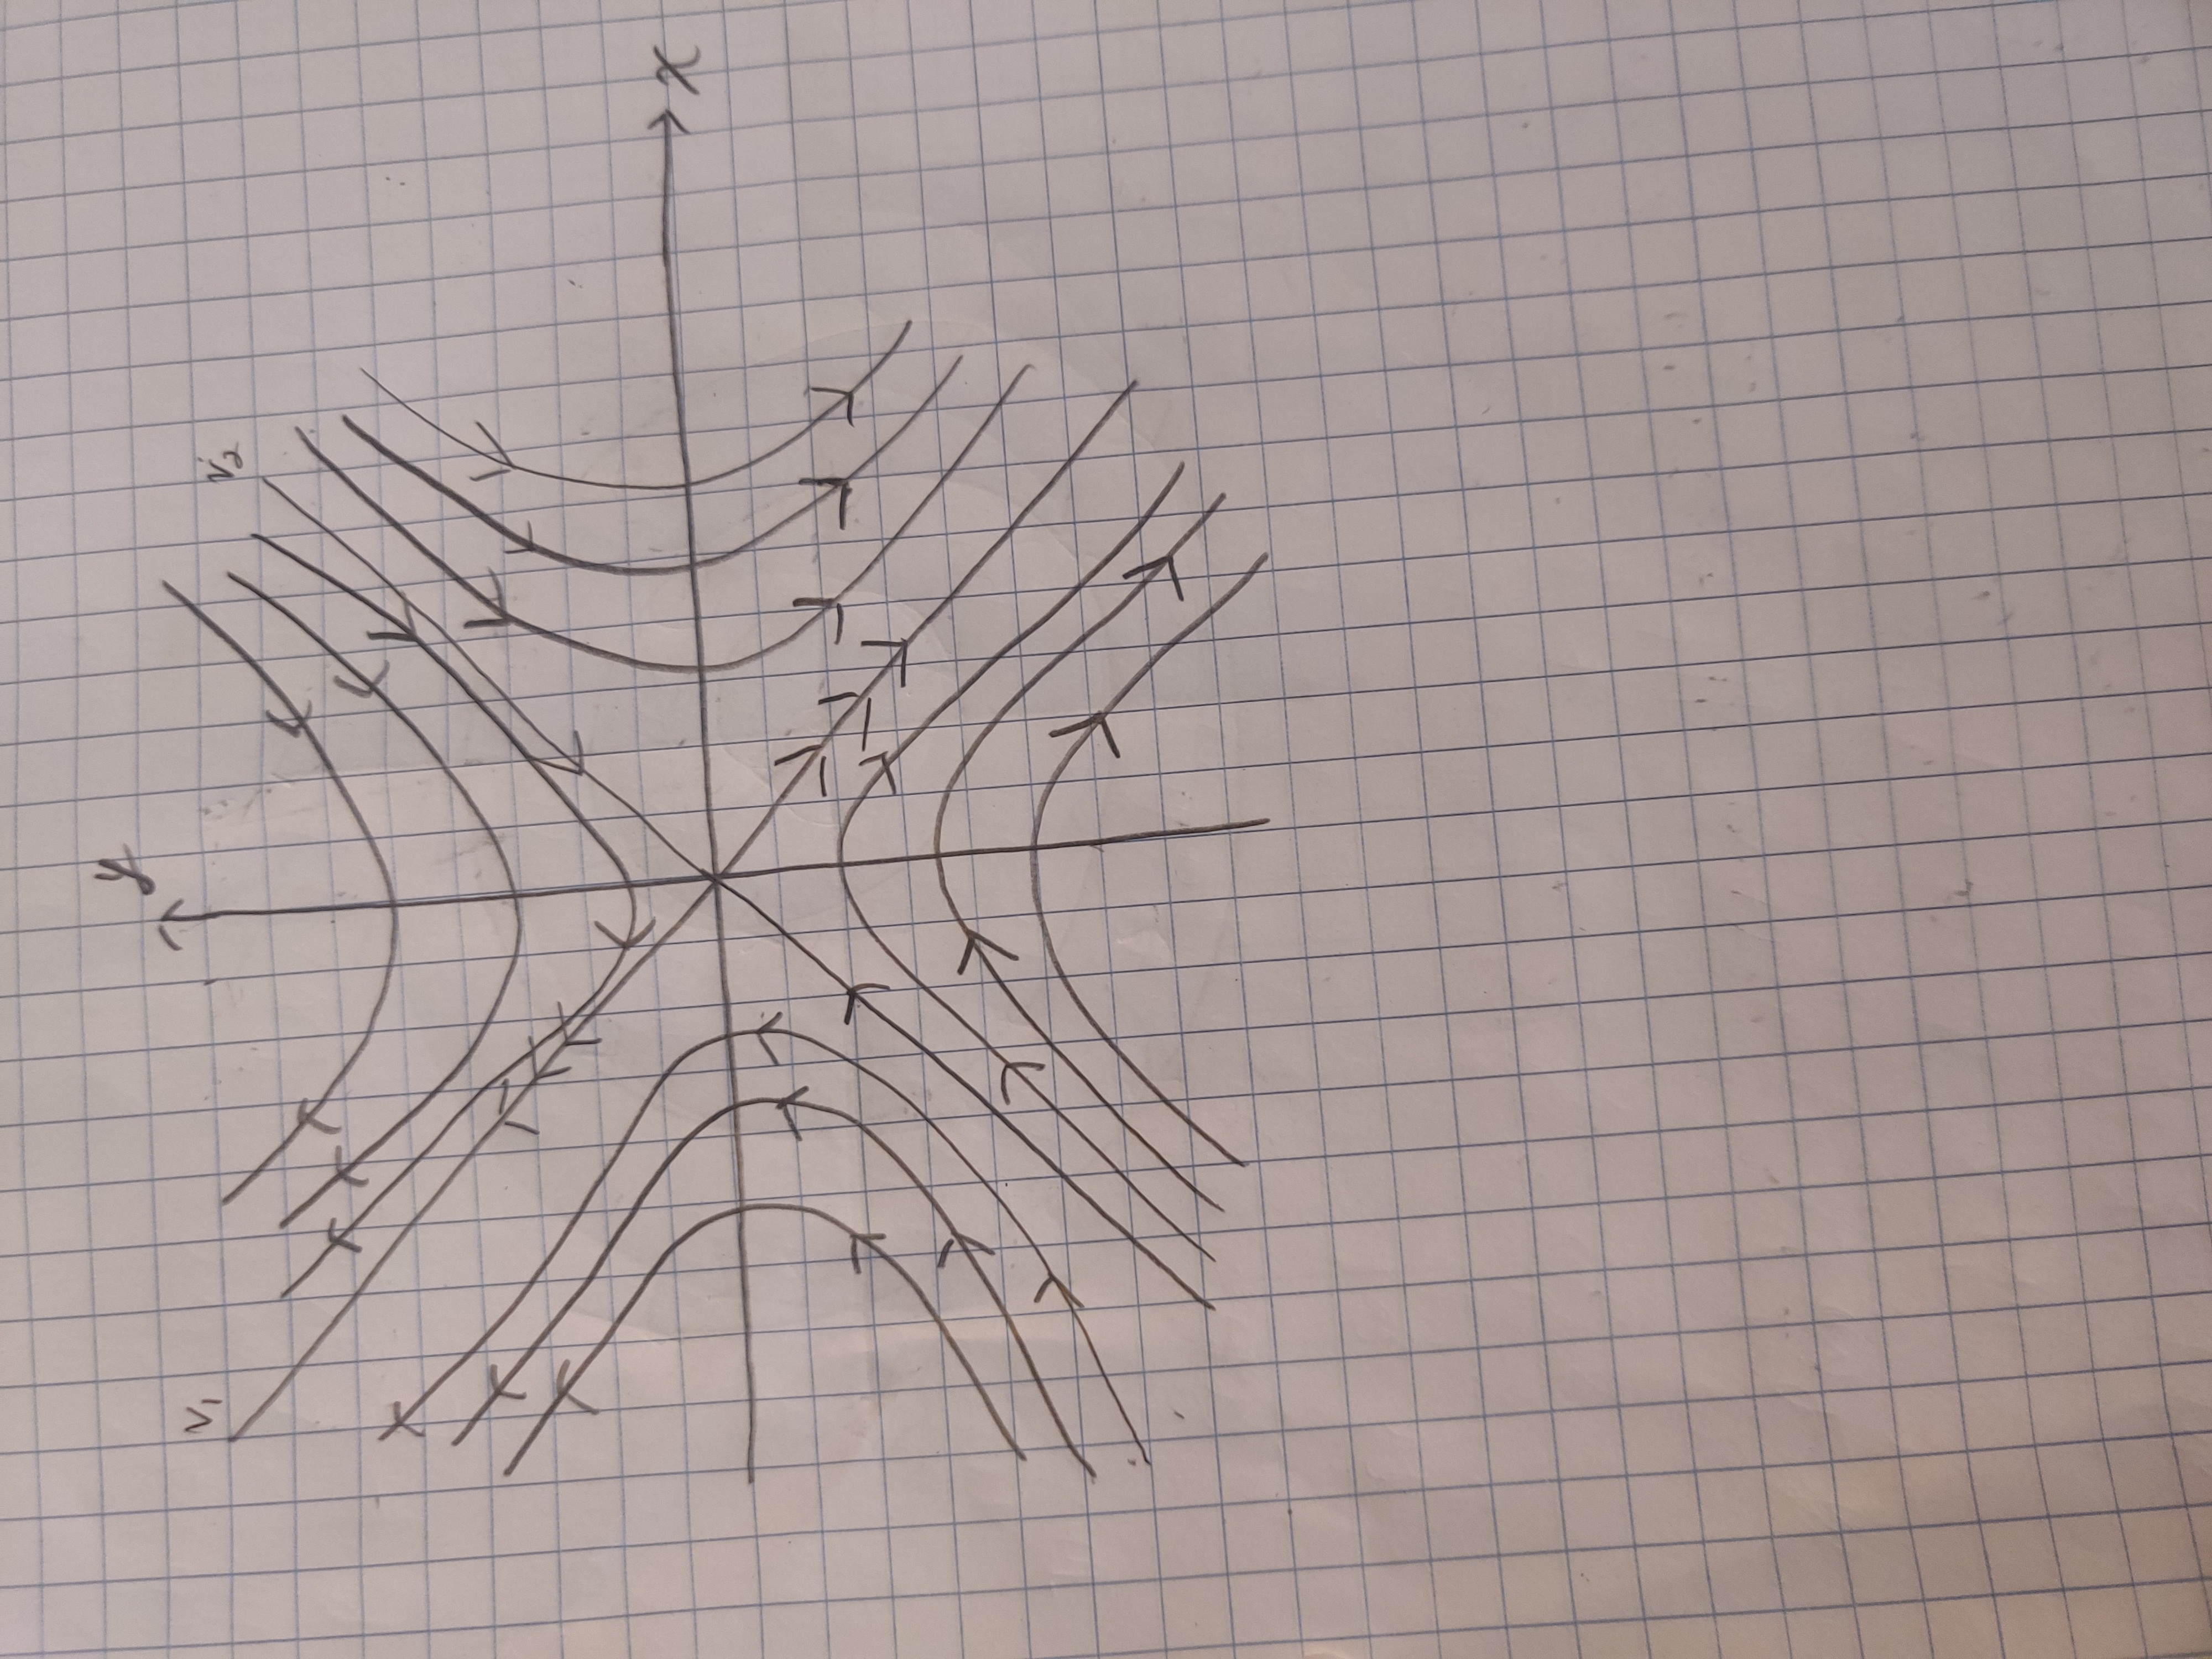
\includegraphics[scale = 0.05]{prob1a_sketch.jpg}
        \end{center}
        Which is supported by the following figure generated by Mathematica:
        \begin{center}
            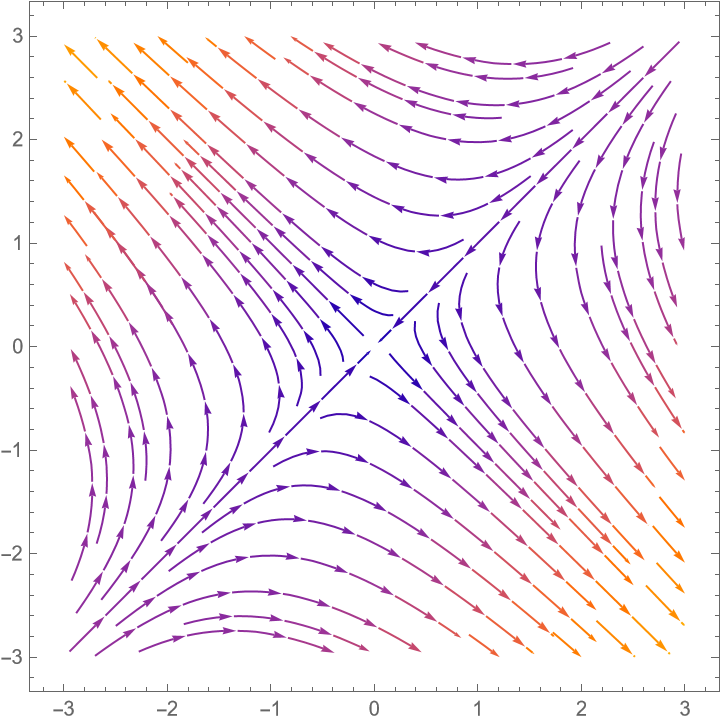
\includegraphics[scale = 0.5]{prob1a_stream.png}
        \end{center}
        \hfill $\mathghost$

        \item[(b)] $A = \begin{pmatrix}
            3 & -2\\
            1 & 1
        \end{pmatrix}$
        \newline\newline
        From Homework 3, we have $\lambda_1 = 2 + i$ and $\lambda_2 = 2 - i$ so that the origin is an unstable spiral since $\text{Re}(\lambda) = 2 > 0$. To determine the orientation, let us write down the system associated with the above matrix:
        \begin{align*}
            \dot{x} &= 3x - 2y\\
            \dot{y} &= x + y
        \end{align*}
        at $(x,y) = (1,0)$, $\dot{x} = 3$, $\dot{y} = 1$, and at $(x,y) = (-1,0)$, $\dot{x} = -3$, $\dot{y} = -1$, so that the spiral has counter-clockwise orientation, as we can see in the following figure:
        \begin{center}
            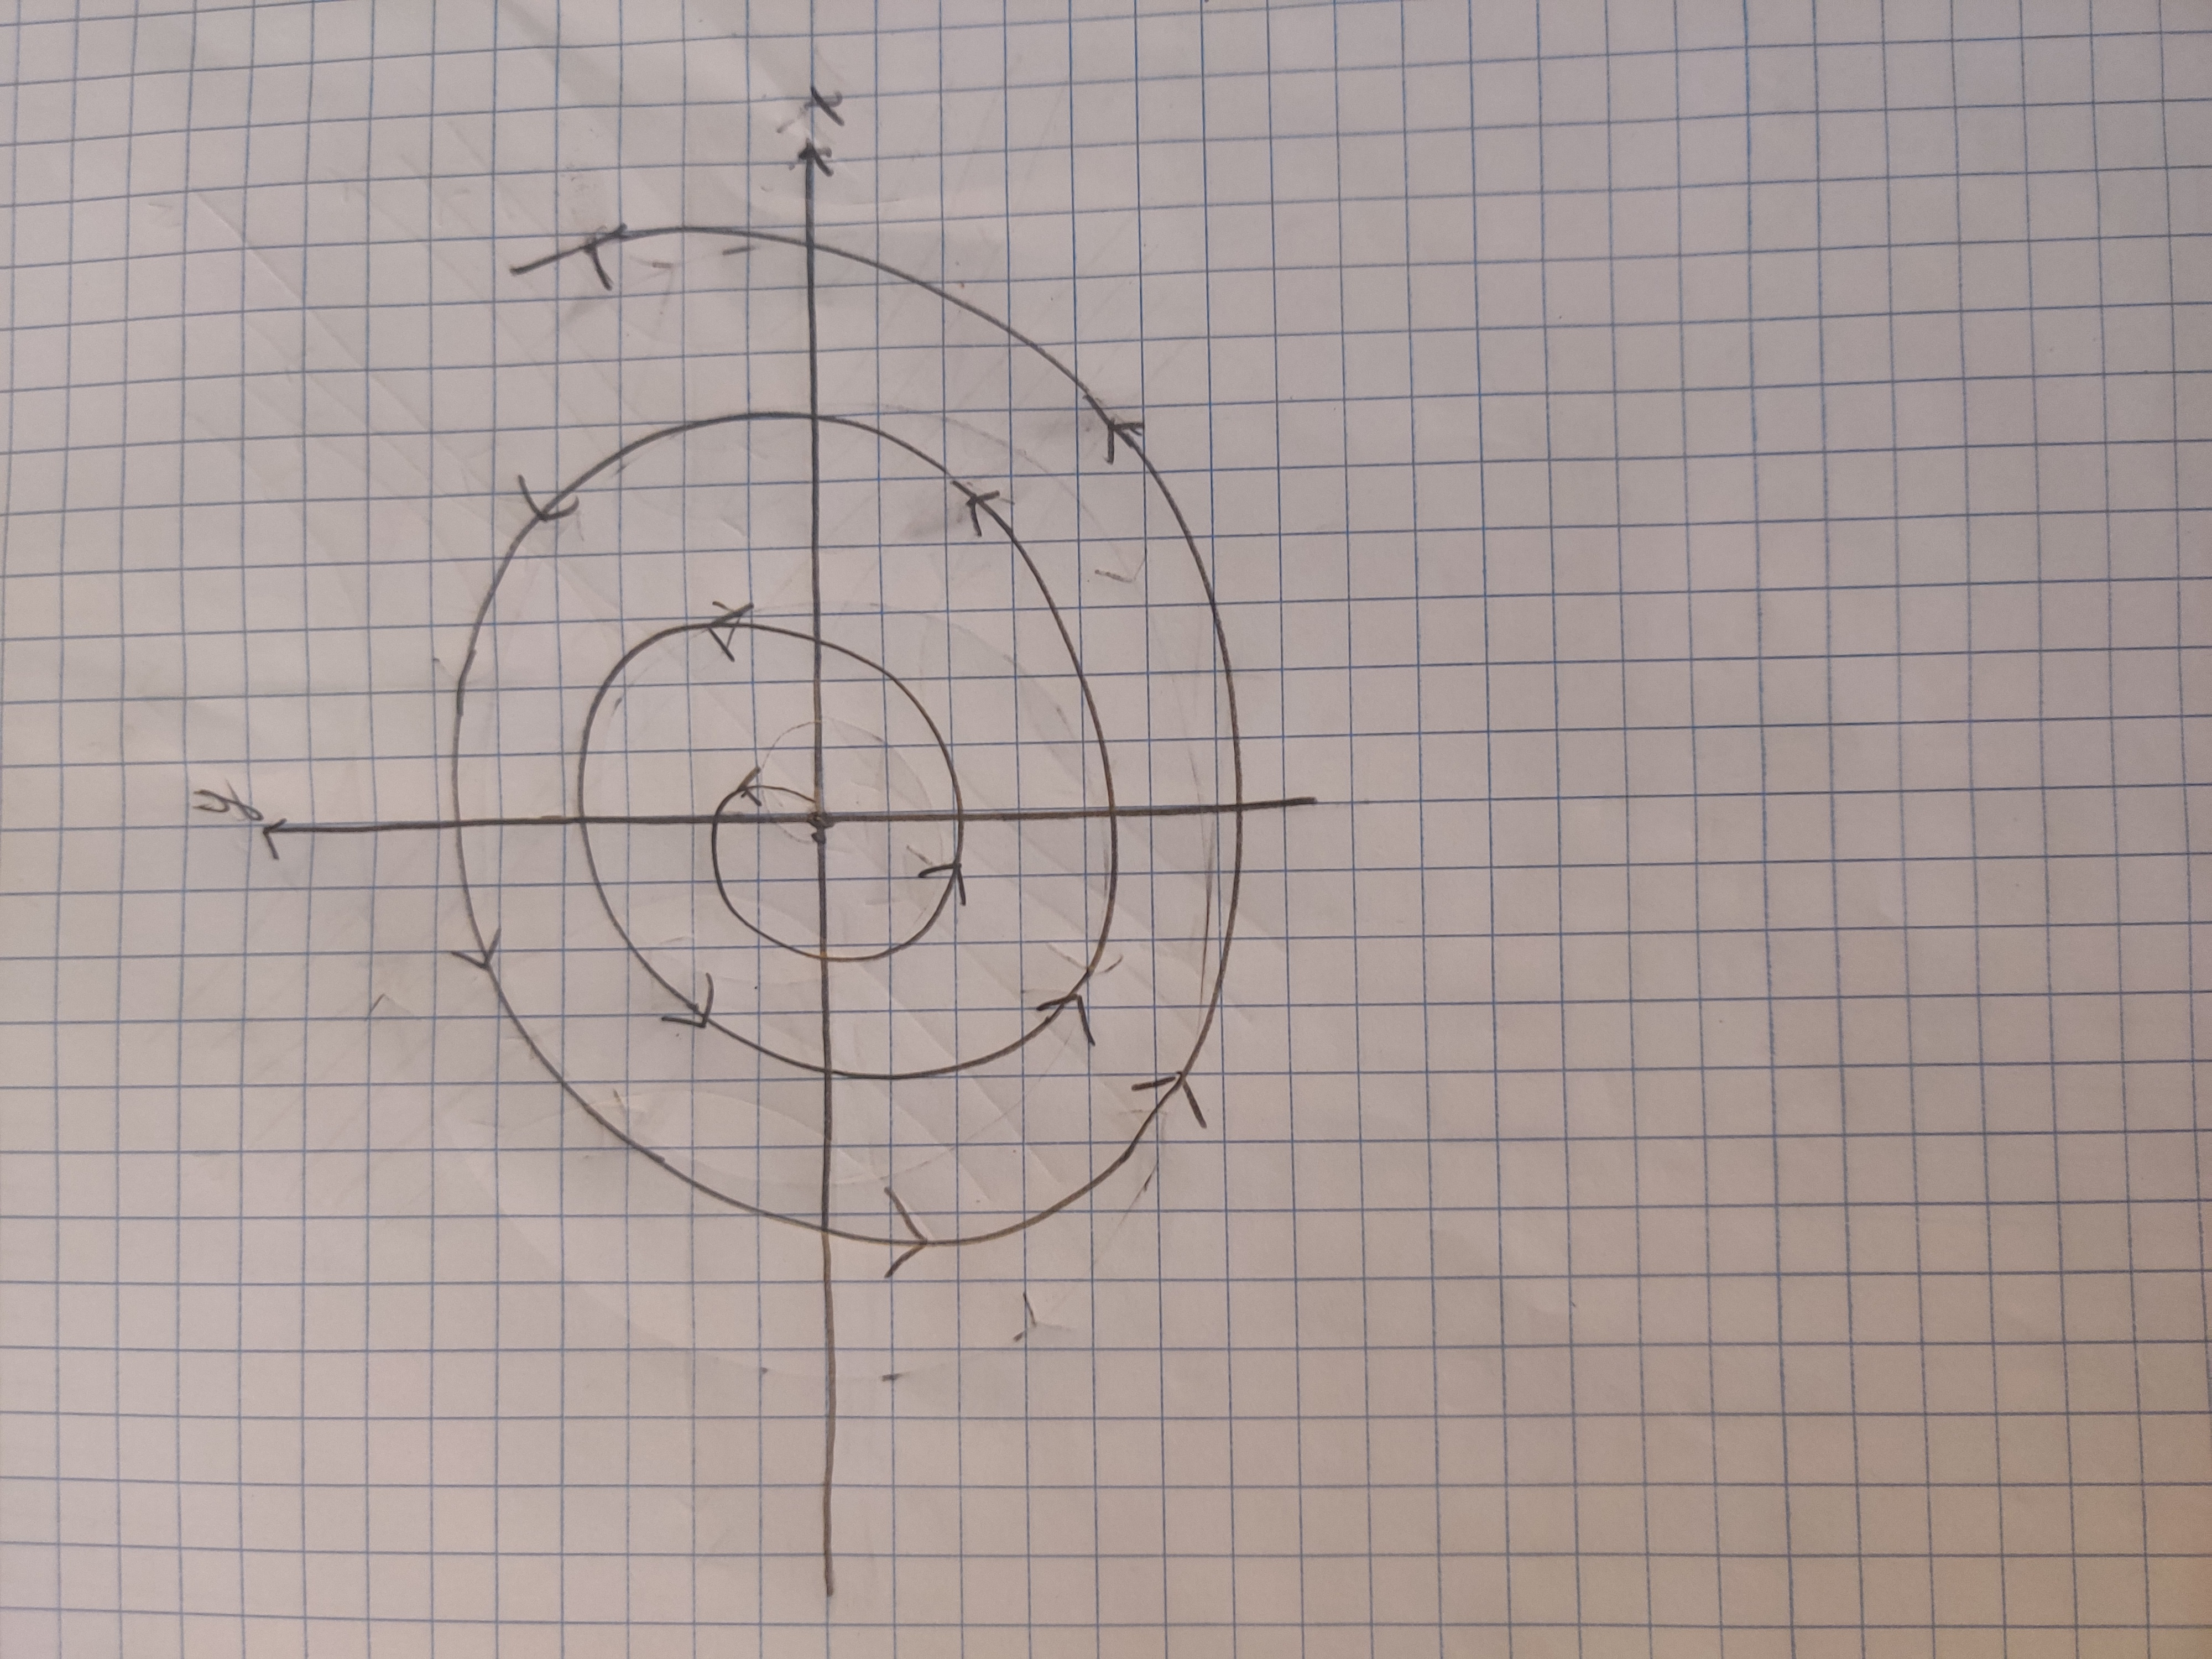
\includegraphics[scale = 0.05]{prob1b_sketch.jpg}
        \end{center}
        Which is supported by the following figure generated by Mathematica:
        \begin{center}
            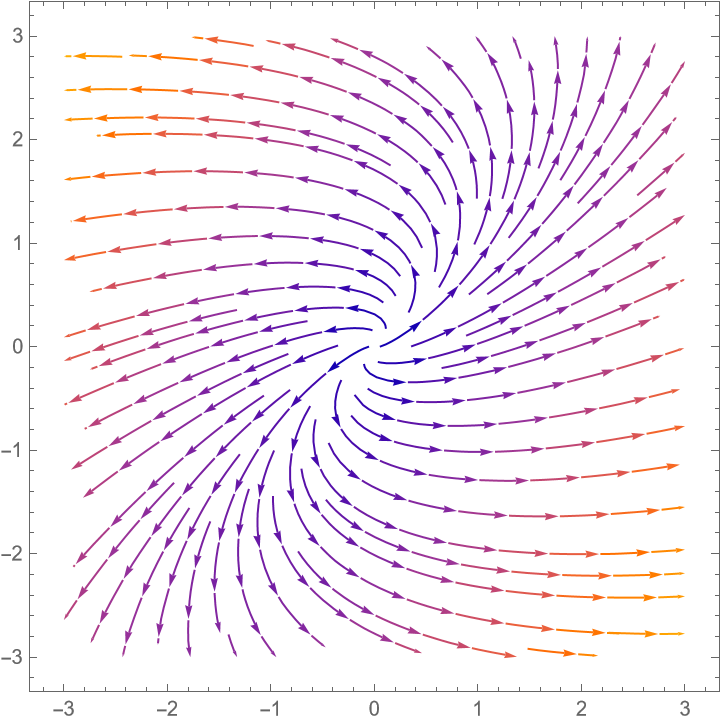
\includegraphics[scale = 0.5]{prob1b_stream.png}
        \end{center}
        \hfill $\mathghost$


        \item[(c)] $A = \begin{pmatrix}
            0 & 1\\
            -1 & 2
        \end{pmatrix}$
        \newline\newline
        From Homework 3, we have $\lambda_1 = \lambda_2 = 1$, so that we have real repeated eigenvalues. The associated eigenvector is
        \[v = \begin{pmatrix}
            1\\
            1
        \end{pmatrix}\]
        So that the origin is an unstable critical point, where any solution $\mathbf{x}(t) \to \pm\infty$ as $t \to \infty$. Additionally, for an initial condition on the line spanned by $v$, the solution will remain on that line and will go to $\pm \infty$ as $t \to \infty$.
        \newline
        Now, if $y = 0$ and $x > 0$, notice $\dot{x} = 0$ and $\dot{y} < 0$ and if $y = 0$ and $x < 0$, $\dot{x} = 0$ and $\dot{y} > 0$. Additionally, taking $y = 1/2$, $x = 1$ (so that we are above the $x-$axis but below the line spanned by $v$), we have $\dot{x} = 1/2$, $\dot{y} = 0$. By a similar analysis for when $x,y < 0$, we have that the solutions near the line spanned by $v$ ``curve around" and go off to $\pm \infty$, as we can see in the below figures:
        \begin{center}
            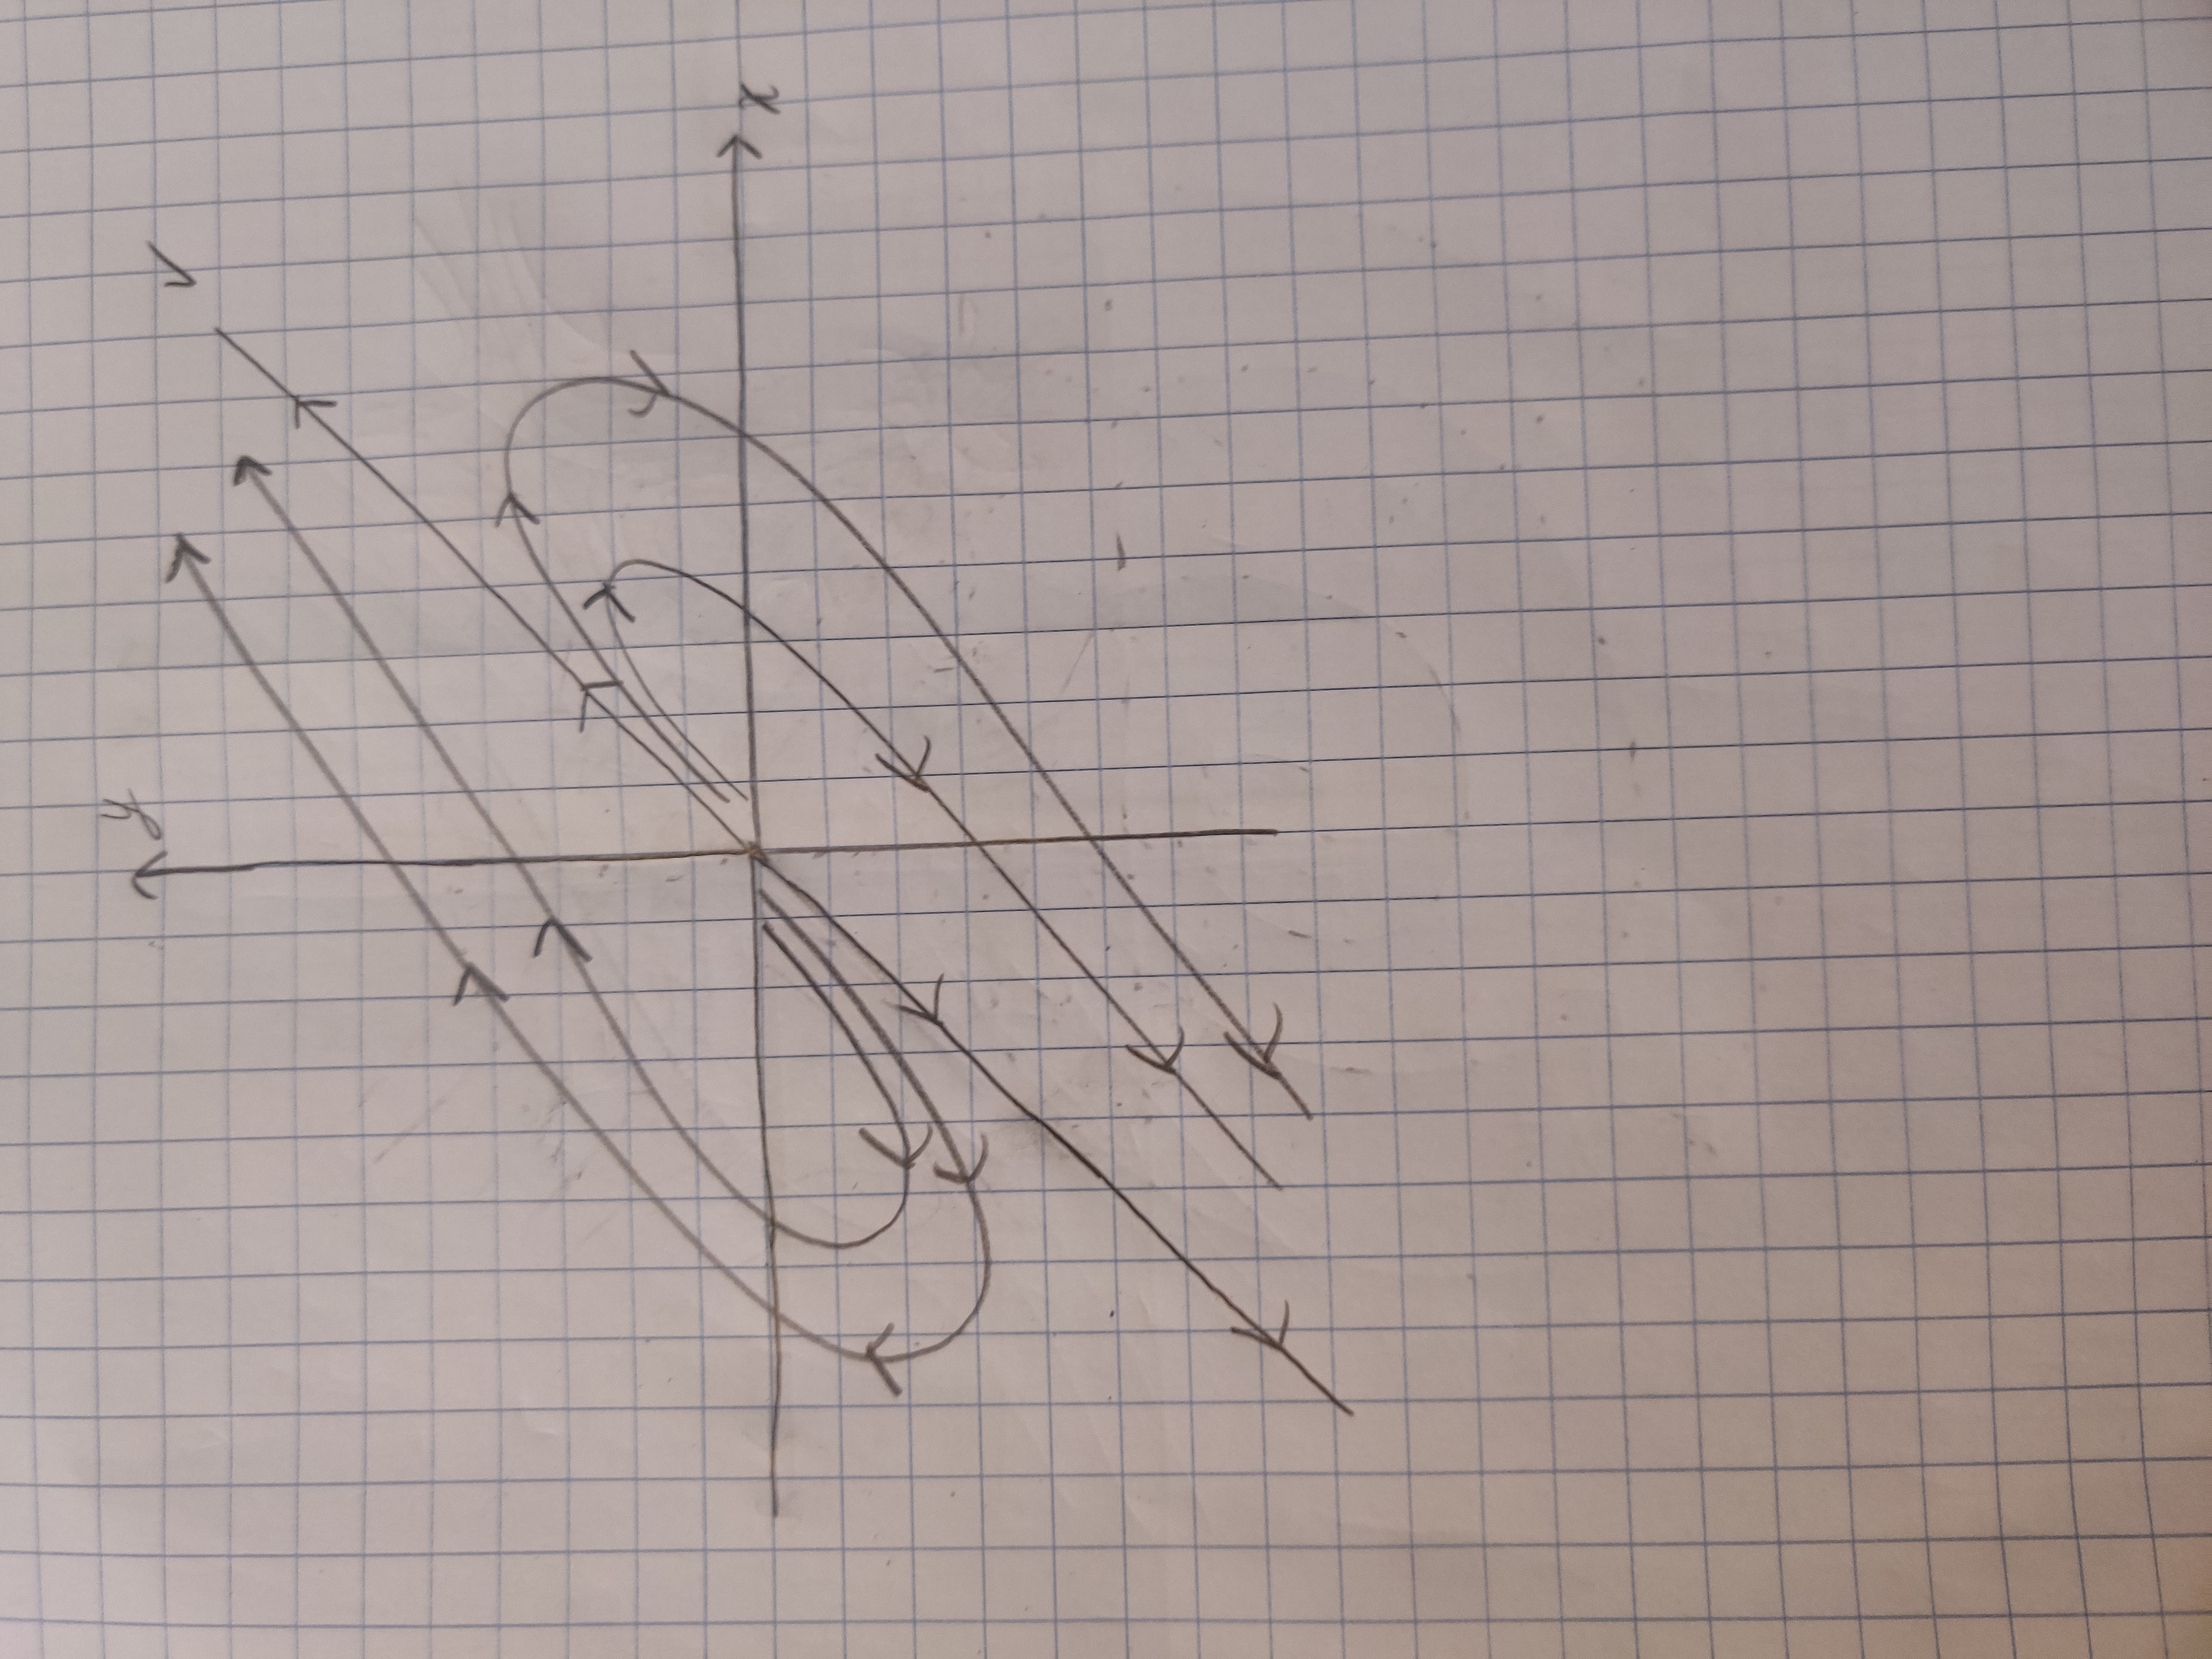
\includegraphics[scale = 0.05]{prob1c_sketch.jpg}
        \end{center}
        which is supported by the following vector plot generated by Mathematica:
        \begin{center}
            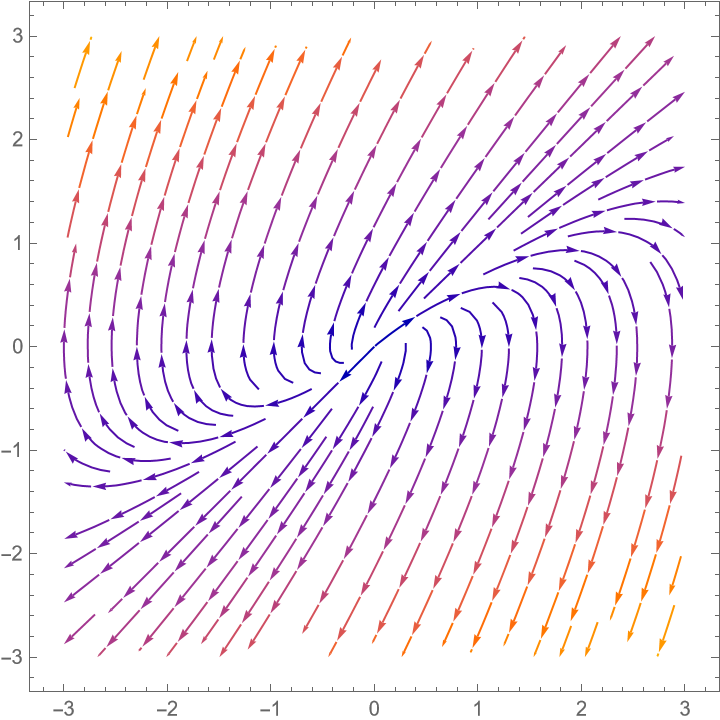
\includegraphics[scale = 0.5]{prob1c_stream.png}
        \end{center}
    \end{itemize}
\end{itemize}
\hfill $\mathghost$
\pagebreak
\section*{Nonlinear Stability}
\begin{itemize}
    \item[2.] Characterize the stability of the following \textit{nonlinear} systems near the critical points. Make a sketch of the vector field near the critical points.
    \begin{itemize}
        \item[(a)] 
        \begin{align*}
            \dot{x} &= x + x^2\\
            \dot{y} &= x + y^2
        \end{align*}
        To begin, let us find the critical points of the system. Beginning with $\dot{x}$:
        \begin{align*}
            \dot{x} &= 0\\
            \implies x + x^2 &= 0\\
            x(1 + x) &= 0\\
            \implies x = 0, \hspace{0.4cm} &x = -1
        \end{align*}
        and now for $\dot{y}$:
        \begin{align*}
            \dot{y} &= 0\\
            \implies x + y^2 &= 0\\
            y^2 &= -x
        \end{align*}
        so that if $x = -1$, $y^2 = 1 \implies y = \pm 1$ and if $x = 0$, $y = 0$. Hence the critical points of the system are 
        \[(-1,-1), \hspace{0.3cm} (-1,1), \hspace{0.3cm} (0,0) \]
        Now let us linearize the system. Let $f(x,y) = x + x^2$ and $g(x,y) = x + y^2$ so that 
        \begin{align*}
            f_x(x,y) &= 1 + 2x\\
            f_y(x,y) &= 0\\
            g_x(x,y) &= 1\\
            g_y(x,y) &= 2y
        \end{align*}
        so that, at the critical point $(-1,-1)$, we have $f_x(-1,-1) = -1$, $f_y = 0$, $g_x = 1$, and $g_y(-1,-1) = -2$. That is, we wish to find the behaviour of the linear system described by the following matrix:
        \[A = \begin{pmatrix}
            -1 & 0\\
            1 & -2
        \end{pmatrix}\]
        finding the eigenvalues:
        \begin{align*}
            \left|\begin{matrix}
                -1 -\lambda & 0\\
                1 & -2 - \lambda
            \end{matrix}\right| &= (\lambda + 2)(\lambda + 1)\\
            &= 0\\
            \implies \lambda_1 = -2, \hspace{0.4cm} &\lambda_2 = -1
        \end{align*}
        so that this critical point is an improper attractive node. Finding the associated eigenvectors:
        \begin{align*}
            \begin{pmatrix}
                -1 - \lambda_1 & 0\\
                1 & -2 - \lambda_1
            \end{pmatrix} &= \begin{pmatrix}
                1 & 0\\
                1 & 0
            \end{pmatrix}.
        \end{align*}
        Hence $v_1 = (0,1)^T$ (when letting the second component be 1). For $\lambda_2$,
        \begin{align*}
            \begin{pmatrix}
                -1 - \lambda_2 & 0\\
                1 & -2 - \lambda_2
            \end{pmatrix} &= \begin{pmatrix}
                0 & 0\\
                1 & -1
            \end{pmatrix}.
        \end{align*}
        And so $v_2 = (1,1)^T$.




        Now, for the critical point $(-1,1)$, $f_x(-1,1) = -1$, $f_y(-1,1) = 0$, and $g_x(-1,1)1$, $g_y(-1,1) = 2$ and so, finding the eigenvalues, we have
        \begin{align*}
            \left|\begin{matrix}
                -1 - \lambda & 0\\
                1 & 2 - \lambda
            \end{matrix}\right| &= (\lambda - 2)(\lambda + 1)\\
            &= 0\\
            \implies \lambda_1 = 2, \hspace{0.5cm} &\lambda_2 = -1
        \end{align*}
        since $\lambda_1 > 0$ and $\lambda_2 < 0$, we have that this critical point is a saddle. Now, finding the eigenvectors for $\lambda_1$ and $\lambda_2$, we have, respectively:
        \begin{align*}
            \begin{pmatrix}
                -1 - \lambda_1 & 0\\
                1 & 2 - \lambda_1
            \end{pmatrix} &= \begin{pmatrix}
                -3 & 0\\
                1 & 0
            \end{pmatrix}
        \end{align*}     
        \begin{align*}
            \begin{pmatrix}
                -1 - \lambda_2 & 0\\
                1 & 2 - \lambda_2
            \end{pmatrix} &= \begin{pmatrix}
                0 & 0\\
                1 & 3
            \end{pmatrix}
        \end{align*}
        so that
        \[v_1 = \begin{pmatrix}
            0\\
            1
        \end{pmatrix} \hspace{0.6cm} v_2 = \begin{pmatrix}
            -3\\
            1
        \end{pmatrix}\]
        

        Finally, for the critical point $(0,0)$, we have $f_x(0,0) = 1$, $f_y(0,0) = 0$, and $g_x(0,0) = 1$, $g_y(0,0) = 0$ so that the matrix that represents the linearized system near this critical point is
        \[A = \begin{pmatrix}
            1 & 0\\
            1 & 0
        \end{pmatrix}\]
        and so, finding the eigenvalues,
        \begin{align*}
            \left|\begin{matrix}
                1 - \lambda & 0\\
                0 & -\lambda
            \end{matrix}\right| &= \lambda(1 - \lambda)\\
            &= 0\\
            \implies \lambda_1 = 0, \hspace{0.5cm} &\lambda_2 = 1.
        \end{align*}
        Thus, this critical point is unstable. Finding the eigenvectors:
        \begin{align*}
            \begin{pmatrix}
                1 - \lambda_1 & 0\\
                1 & -\lambda_1
            \end{pmatrix} &= \begin{pmatrix}
                1 & 0\\
                1 & 0
            \end{pmatrix}
        \end{align*}
        \begin{align*}
            \begin{pmatrix}
                1 -\lambda_2 & 0\\
                1 & -\lambda_2
            \end{pmatrix} &= \begin{pmatrix}
                0 & 0\\
                1 & -1
            \end{pmatrix}
        \end{align*}
        so that our associated eigenvectors are, respectively,
        \[v_1 = \begin{pmatrix}
            0\\
            1
        \end{pmatrix}, \hspace{0.6cm} v_2 = \begin{pmatrix}
            1\\
            1
        \end{pmatrix}\]
       
        All together, the behavior of this nonlinear system looks approximately like:
        \begin{center}
            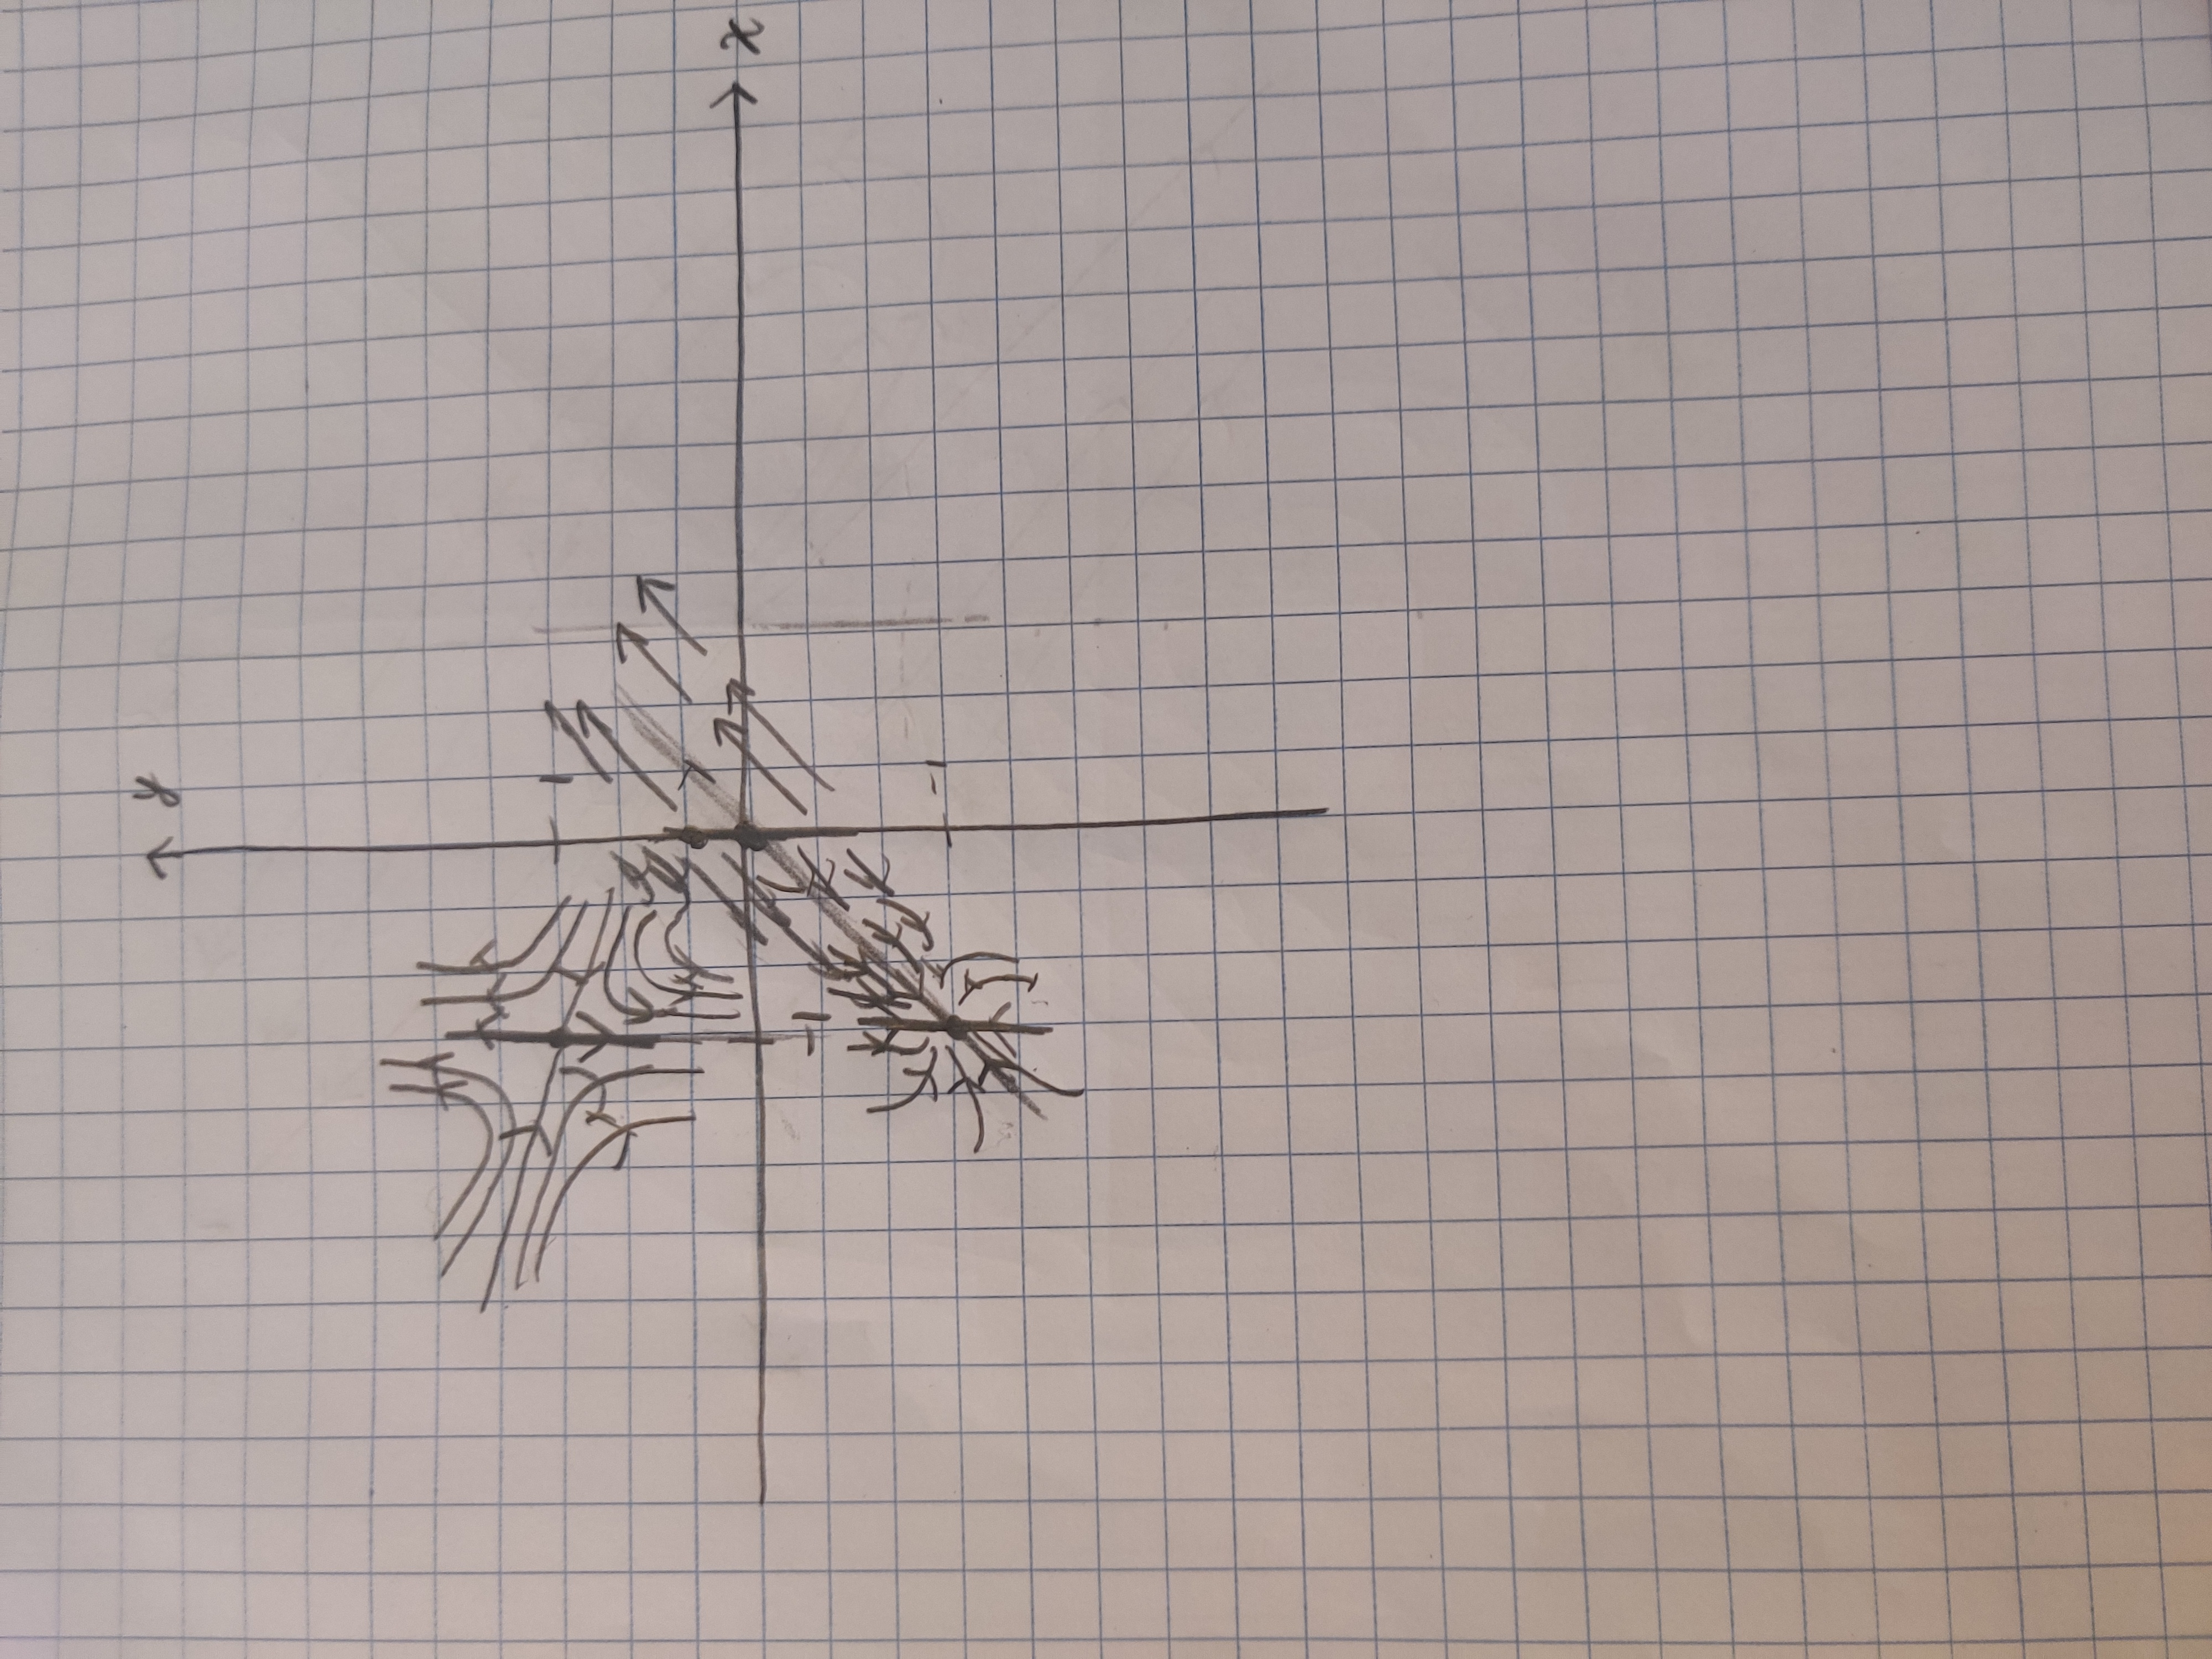
\includegraphics[scale = 0.05]{prob2a_sketch.jpg}
        \end{center}
        which is supported the following figure generated by Mathematica:
        \begin{center}
            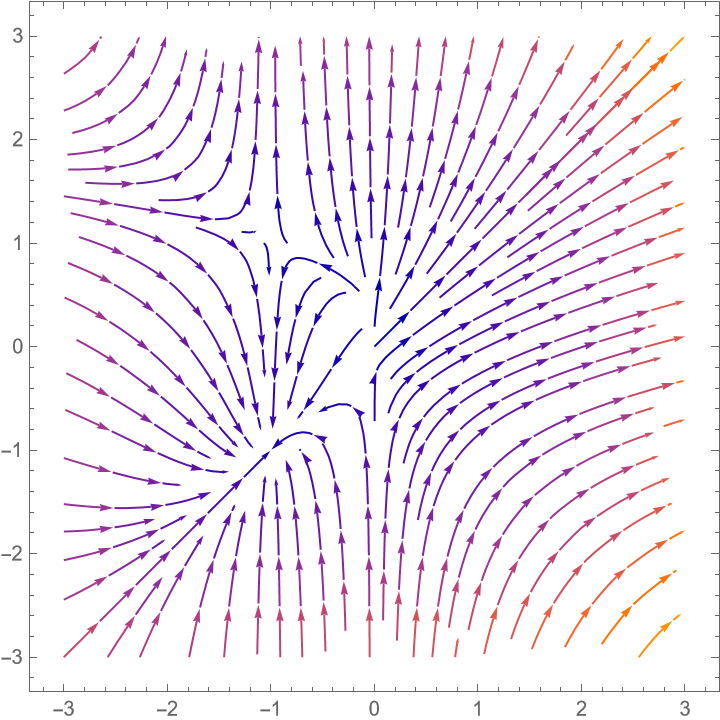
\includegraphics[scale = 0.5]{prob2a_stream.png}
        \end{center}
        \hfill $\mathghost$
    

        
        \item[(b)] 
        \begin{align*}
            \dot{x} &= x(3 - x - y)\\
            \dot{y} &= y(x - y - 1)
        \end{align*}
        Let us begin by finding the critical points:
        \begin{align*}
            \dot{x} &= 0\\
            \implies x(3 - x - y) &= 0\\
            \implies x = 0 \hspace{0.3cm} \text{ or }& \hspace{0.3 cm} x = 3 - y
        \end{align*}
        and
        \begin{align*}
            \dot{y} &= 0\\
            \implies y(x - y - 1) &= 0\\
            \implies y = 0 \hspace{0.3cm} \text{ or }& \hspace{0.3cm} y = x - 1
        \end{align*}
        thus, if $x = 0$, we have that either $y = 0$ or $y = -1$. Additionally, if $y = 0$, we have $x = 3$. Finally, if $x = 3 - y$ and $y = x - 1$, we have $y = 1$ and $x = 2$ so that our critical points are
        \[(0,0), \hspace{0.25cm} (0,-1), \hspace{0.25cm} (3,0), \hspace{0.25cm} (2,1).\]
        Now, let $f(x,y) = x(3 - x - y)$ and $g(x,y) = y(x - y - 1)$ so that 
        \begin{align*}
            f_x(x,y) &= 3 - 2x - y\\
            f_y(x,y) &= -x
        \end{align*}
        and
        \begin{align*}
            g_x(x,y) &= y\\
            g_y(x,y) &= x - 2y - 1.
        \end{align*}
        Now, linearizing near the critical point $(0,0)$, we have $f_x(0,0) = 3$, $f_y(0,0) = 0$, and $g_x(0,0) = 0$, $g_y(0,0) = -1$. Thus we wish to find the behavior of the system described by
        \[A = \begin{pmatrix}
            3 & 0\\
            0 & -1
        \end{pmatrix}.\]
        Clearly, $\lambda_1 = 3$ and $\lambda_2 = -1$ with associated eigenvectors
        \[v_1 = \begin{pmatrix}
            1\\
            0
        \end{pmatrix}, \hspace{0.4cm} v_2 = \begin{pmatrix}
            0\\
            1
        \end{pmatrix}\]
        and since $\lambda_1 > 0$, $\lambda_2 < 0$, we have that this critical point is a saddle.
        \newline\newline
        Now, at the critical point $(0,-1)$, $f_x(0,-1) = 4$, $f_y(0,-1) = 0$, and $g_x(0,-1) = -1$, $g_y(0,1) = 1$. Thus we wish to find the behavior of the system described by
        \[A = \begin{pmatrix}
            4 & 0\\
            -1 & 1
        \end{pmatrix}.\]
        Beginning with the eigenvectors, we have
        \begin{align*}
            \left|\begin{matrix}
                4 - \lambda & 0\\
                -1 & 1 - \lambda
            \end{matrix}\right| &= (4 - \lambda)(1 -\lambda)\\
            &= 0\\
            \implies \lambda_1 = 4, \hspace{0.3cm}& \lambda_2 = 1.
        \end{align*}
        Hence this critical point is an improper, repulsive node. Finding the associated eigenvectors for $\lambda_1, \lambda_2$, respectively, we find
        \begin{align*}
            \begin{pmatrix}
                4 - \lambda_1 & 0\\
                -1 & 1 - \lambda_1
            \end{pmatrix} &= \begin{pmatrix}
                0 & 0\\
                -1 & -3
            \end{pmatrix}
        \end{align*}
        and
        \begin{align*}
            \begin{pmatrix}
                4 - \lambda_2 & 0\\
                -1 & 1 - \lambda_2
            \end{pmatrix} &= \begin{pmatrix}
                3 & 0\\
                -1 & 0
            \end{pmatrix}
        \end{align*}
        so that
        \[v_1 = \begin{pmatrix}
            -3\\
            1
        \end{pmatrix}, \hspace{0.5cm} v_2 = \begin{pmatrix}
            0\\
            1
        \end{pmatrix}\]
       
        At the critical point $(3,0)$, we have $f_x(3,0) = -3$, $f_y(3,0) = -3$, and $g_x(3,0) = 2$, $g_y(3,0) = 2$. Thus we wish to find the behavior of the system described by 
        \[A = \begin{pmatrix}
            -3 & -3\\
            0 & 2
        \end{pmatrix}.\]
        Finding the eigenvalues:
        \begin{align*}
            \left|\begin{matrix}
                -3 - \lambda & -3\\
                0 & 2 - \lambda
            \end{matrix}\right| &= (\lambda - 2)(\lambda + 3)\\
            &= 0\\
            \implies \lambda_1 = 2, \hspace{0.5cm}& \lambda_2 = -3
        \end{align*}
        thus this critical point is a saddle. Finding the associated eigenvectors:
        \begin{align*}
            \begin{pmatrix}
                -3 - \lambda_1 & -3\\
                0 & 2 - \lambda_1
            \end{pmatrix} &= \begin{pmatrix}
                -5 & -3\\
                0 & 0
            \end{pmatrix}
        \end{align*}
        and
        \begin{align*}
            \begin{pmatrix}
                -3 - \lambda_2 & -3\\
                0 & 2 - \lambda_2
            \end{pmatrix} &= \begin{pmatrix}
                0 & -3\\
                0 & 5
            \end{pmatrix}
        \end{align*}
        we have
        \[v_1 = \begin{pmatrix}
            -3\\
            5
        \end{pmatrix}, \hspace{0.5cm} v_2 = \begin{pmatrix}
            1\\
            0
        \end{pmatrix}.\]
        
        Finally, at the critical point $(2,1)$, we have $f_x(2,1) = -2$, $f_y(2,1) = -2$, and $g_x(2,1) = 1$, $g_y(2,1) = -1$. Thus we wish to find the behavior of the system described by 
        \[A = \begin{pmatrix}
            -2 & -2\\
            1 & -1
        \end{pmatrix}.\]
        Finding the eigenvalues:
        \begin{align*}
            \left|\begin{matrix}
                -2-\lambda & -2\\
                1 & -1-\lambda
            \end{matrix}\right| &= (\lambda + 1)(\lambda + 2) + 2\\
            &= \lambda^2 + 3\lambda + 4 = 0
        \end{align*}
        so 
        \[\lambda = \frac{-3 \pm i\sqrt{7}}{2}.\]
        So we have complex eigenvalues with negative real parts, meaning that this critical point is a stable spiral. To determine the orientation of the spiral, check the points $(3,1)$ and $(1,1)$:
        \begin{align*}
            \dot{y}|_{(3,1)} &= 1\\
            \dot{y}|_{(1,1)} &= -1
        \end{align*}
        so that the orientation is counter-clockwise.
        \newline
        Putting it together, we have the phase portrait for the nonlinear system:
        \begin{center}
            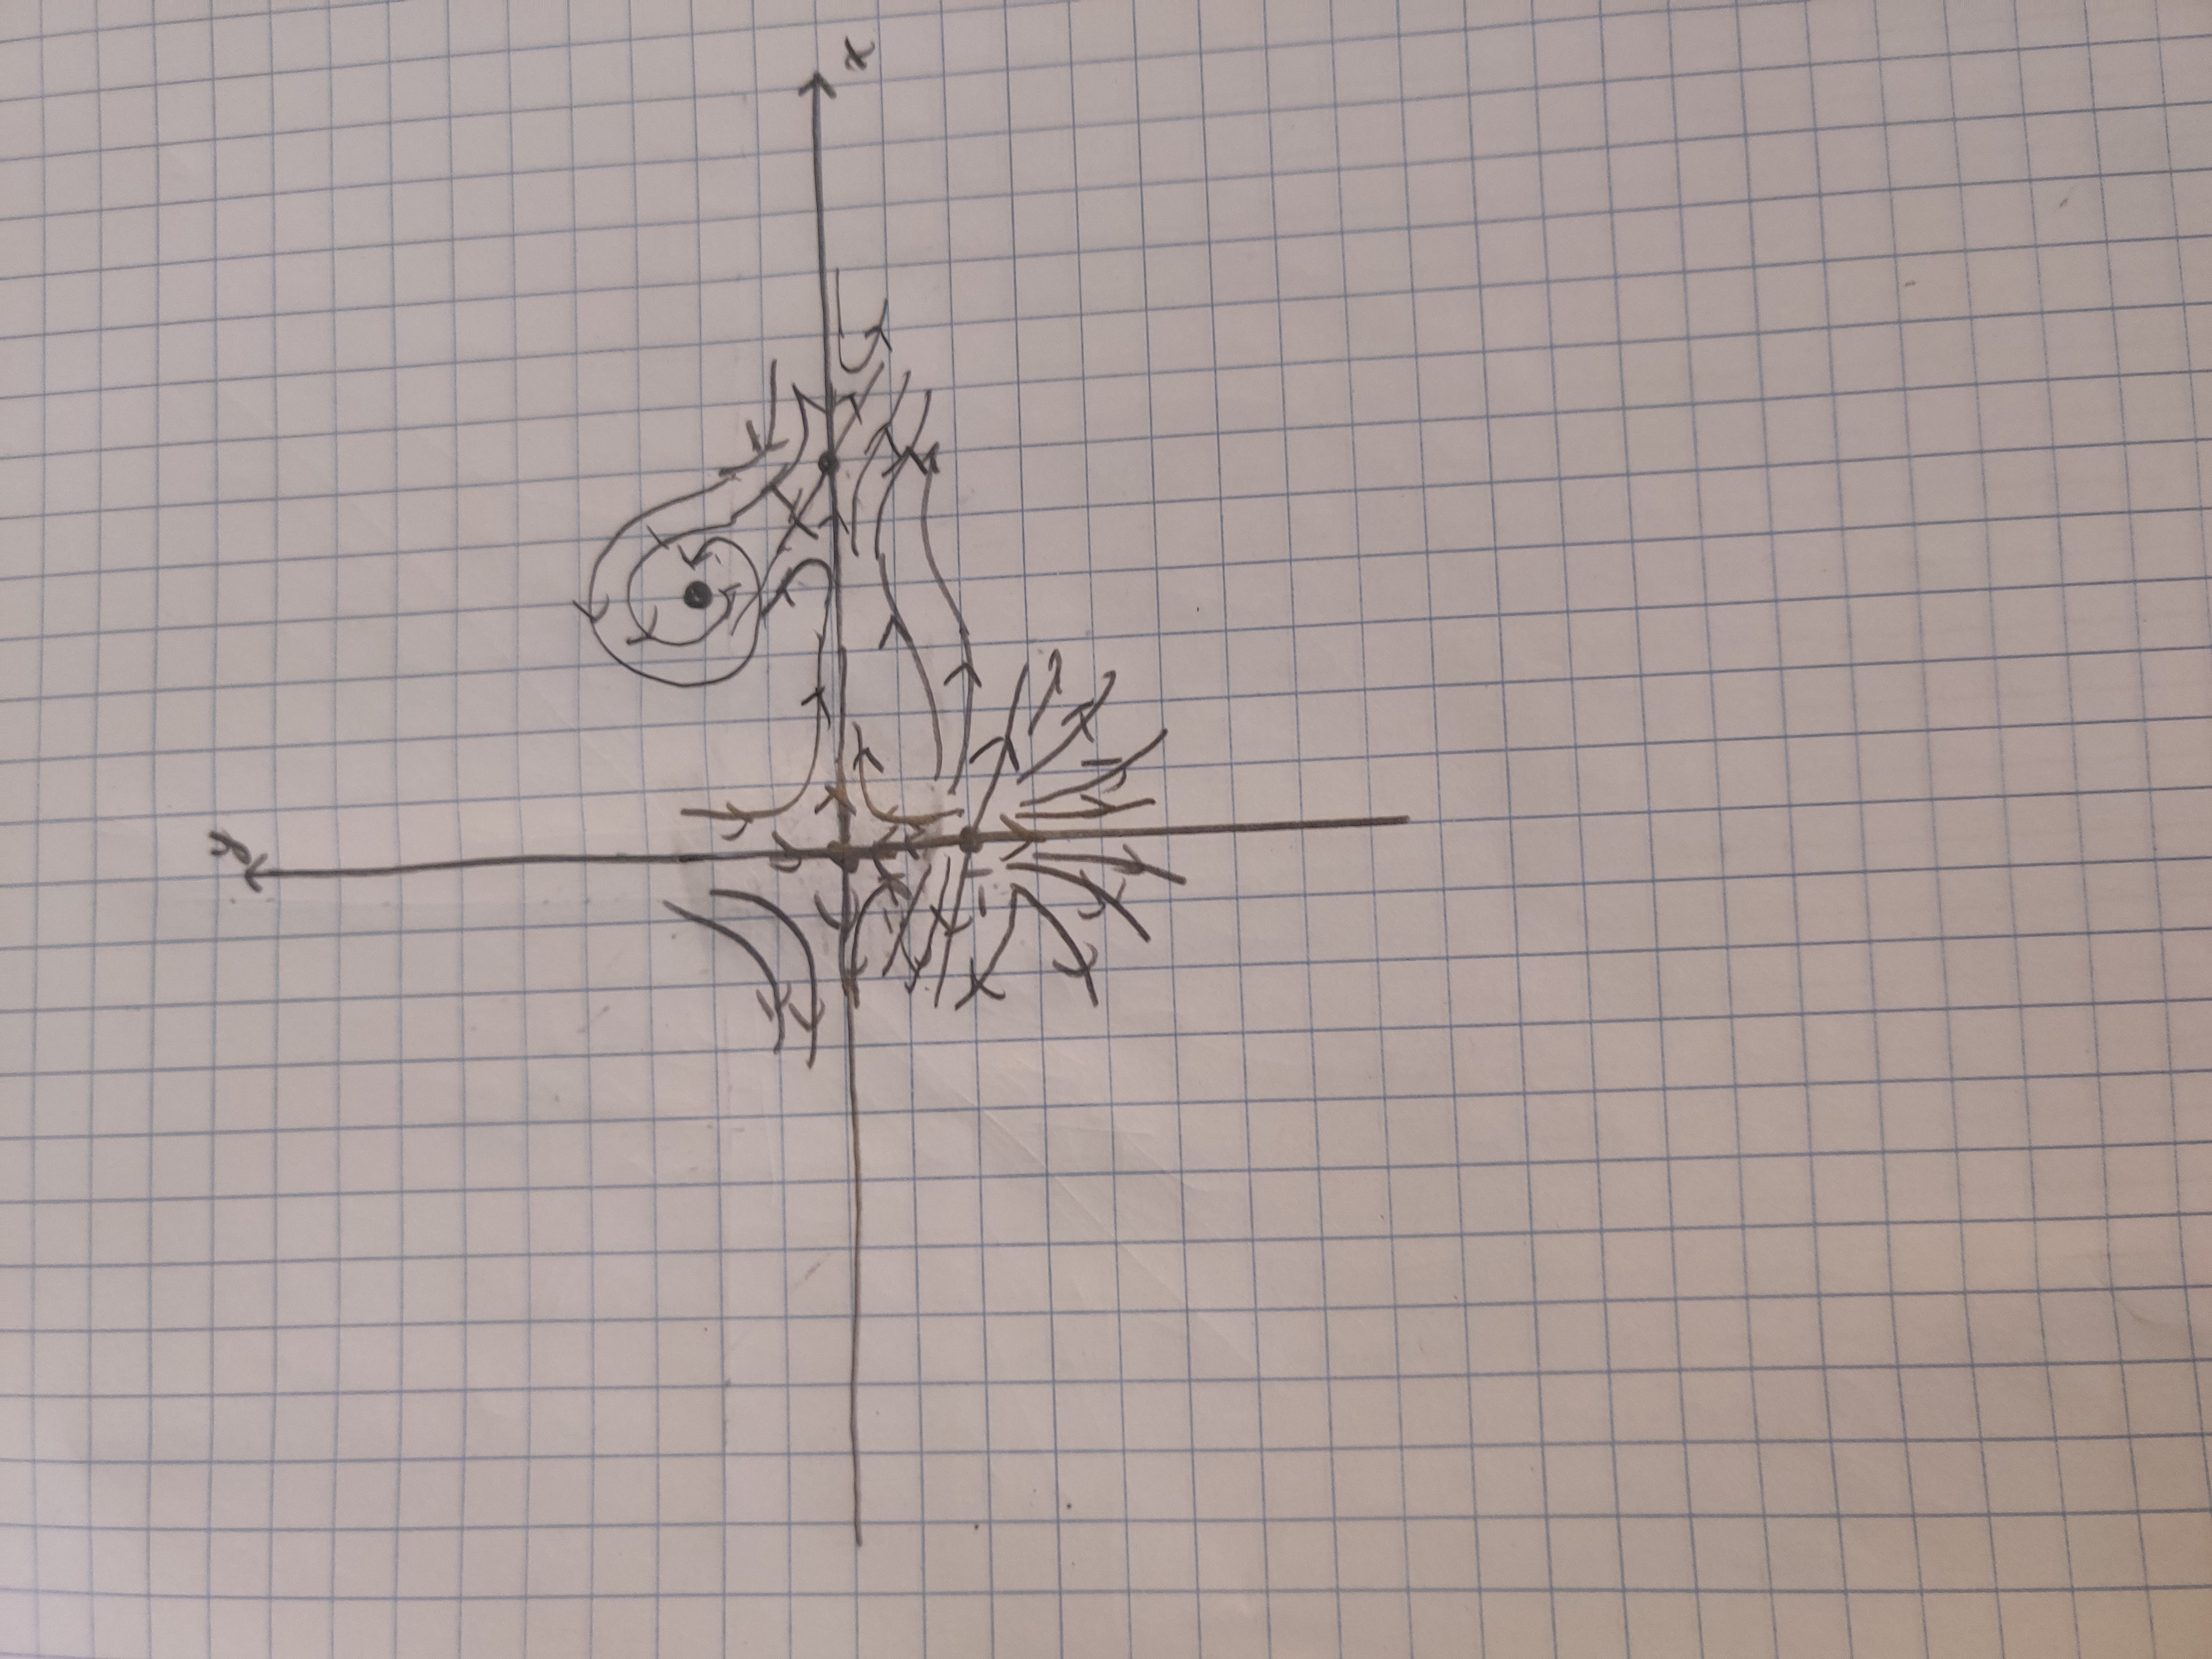
\includegraphics[scale = 0.05]{prob2b_sketch.jpg}
        \end{center}
        which is supported by the following vector plot generated by Mathematica:
        \begin{center}
            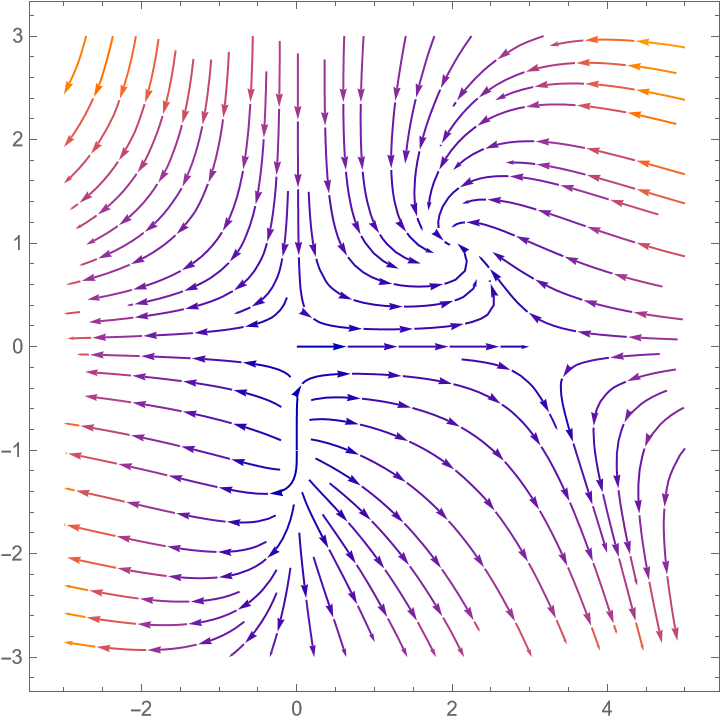
\includegraphics[scale = 0.5]{prob2b_stream.png}
        \end{center}
        
    \end{itemize}
\end{itemize}
\hfill $\mathghost$
\pagebreak
\section*{Liapunov Stability}
\begin{itemize}
    \item[3.] Consider the system 
    \begin{align*}
        \dot{x} &= -x + y + xy\\
        \dot{y} &= x - y - x^2
    \end{align*}
    Find an appropriate Liapunov function to show that the origin is asymptotically stable and every initial condition converges to the origin.
    \textit{Soln.} Consider the function $C(t) = x(t)^2 + y(t)^2$. Then
    \begin{align*}
        \dot{C}(t) &= 2x(t)\dot{x}(t) + 2y(t)\dot{y}(t)\\
        &= 2x(-x + y + xy) + 2y(x - y - x^2)\\
        &= -2x^2 + 2xy + 2x^2y + 2xy - 2y^2 - 2x^2y\\
        &= -2x^2 + 4xy - 2y^2\\
        &= -2(x^2 - 2xy + y^2)\\
        &= -2(x - y)^2 \leq 0
    \end{align*}
    hence,
    \[0 \leq C(t) \leq C_0\]
    so that solutions remain stable and bounded. \hfill $\mathghost$
    \pagebreak
    \item[4.] Show that $V(x,y) = x^2 + y^2$ is a Liapunov function for the system
    \[\dot{x} = -\xi x + y, \hspace{0.5cm} \dot{y} = -x - \eta y\]
    where $\xi, \eta > 0$ and investigate the stability of $(x_0, y_0) = (0,0)$.
    \newline\newline
    \textit{Proof:} Begin by noticing that $V(x,y)$ is positive definite. Now,
    \begin{align*}
        \nabla V(x,y) &= \begin{pmatrix}
            2x\\
            2y
        \end{pmatrix}
    \end{align*}
    and so
    \begin{align*}
        \nabla V \cdot \dot{\vec{x}} &= (2x,2y)\begin{pmatrix}
            -\xi x + y\\
            -x - \eta y
        \end{pmatrix}\\
        &= -2\xi x^2 + 2xy - 2xy - 2\eta y^2\\
        &= -2\xi x^2 - 2\eta y^2\\
        &\leq -2\min\{\xi, \eta\}(x^2 + y^2)\\
        &= -2\min\{\xi, \eta\}V\\
        \implies \nabla V \cdot \dot{\vec{x}} &\leq kV
    \end{align*}
    where $k = -2\min\{\xi, \eta\} < 0$. Hence, $V$ is a Liapunov function for the system. I claim that the point $(x_0,y_0) = (0,0)$ is asymptotically stable. To see this, notice
    \begin{align*}
        \nabla V \cdot \dot{\vec{x}} - kV &\leq 0\\
        e^{-kt}\nabla V \cdot \dot{\vec{x}} - ke^{-kt}V &\leq 0\\
        \frac{d}{dt}\left(e^{-kt}V(\vec{x})\right) &\leq 0\\
        \implies e^{-kt}V(\vec{x}) &\leq V_0e^{-kt_0}\\
        \implies V(\vec{x}) &\leq V_0e^{k(t - t_0)}
    \end{align*}
    and since $k < 0$, as $t \to \infty$, $V \to 0$ and hence the origin is asymptotically stable.
    \hfill $\mathghost$
    
    
\end{itemize}
\pagebreak
\section*{Section 3.3 (from textbook)}
\begin{itemize}
    \item[5.] Solve the following differential equations:
    \begin{itemize}
        \item[(i)] $\ddot{x} + 3\dot{x} + 2x = \sinh(t)$.
        \newline\newline
        \textit{Soln.} Let us begin by solving the homogeneous problem:
        \[\ddot{x_h} + 3\dot{x_h} + 2x_h = 0.\]
        Since this is a linear second order homogeneous equation, from the characteristic equation
        \begin{align*}
            r^2 + 3r + 2 &= 0\\
            (r + 2)(r + 1) &= 0\\
            \implies r &= -2,-1
        \end{align*}
        so that the solution to the homogeneous equation is
        \[x_h = C_1e^{-2t} + C_2e^{-t}.\]
        For the particular solution, notice $\sinh(t) = \tfrac{1}{2}(e^t - e^{-t})$ and so, since $e^{-t}$ appears in the homogeneous equation, we will use the ansatz
        \[x_p = Ae^t + Bte^{-t}.\]
        Then
        \begin{align*}
            \dot{x_p} &= Ae^t + Be^{-t} - Bte^{-t}\\
            \ddot{x_p} &= Ae^t - 2Be^{-t} + Bte^{-t}
        \end{align*}
        so that
        \begin{align*}
            \ddot{x_p} + 3\dot{x_p} + 2x_p &= 6Ae^t + 2Be^{-t}\\
            &= \frac{1}{2}e^t - \frac{1}{2}e^{-t}\\
            \implies A = \frac{1}{12}, \hspace{0.5cm}& B = -\frac{1}{2}.
        \end{align*}
        Hence, the solution to this differential equation is
        \[x(t) = C_1e^{-2t} + (C_2 - \tfrac{t}{2})e^{-t} + \tfrac{1}{12}e^t\]
        \hfill $\mathghost$


        \item[(ii)] $\ddot{x} + 2\dot{x} + 2x = \exp(t)$.
        \newline\newline
        \textit{Soln.} Let us begin by solving the homogeneous equation:
        \[\ddot{x_h} + 2\dot{x_h} + 2x_h = 0.\]
        Since this is a second order linear homogeneous equation, we have from the characteristic equation
        \begin{align*}
            r^2 + 2r + 2 &= 0\\
            \implies r &= \frac{-2 \pm \sqrt{4 - 4(1)(2)}}{2}\\
            &= \frac{-2 \pm 2i}{2}\\
            &= -1 \pm i
        \end{align*}
        so that the homogeneous equation is given by
        \[x_h(t) = e^{-t}(C_1\cos(t) + C_2\sin(t)).\]
        Now, for the particular solution, use the ansatz $x_p(t) = Ae^t$, so that
        \begin{align*}
            \dot{x_p} &= Ae^t\\
            \ddot{x_p} &= Ae^t
        \end{align*}
        and so
        \begin{align*}
            \ddot{x_p} + 2\dot{x_p} + 2x_p &= 5Ae^t\\
            \implies A &= \frac{1}{5}
        \end{align*}
        so that the solution to the differential equation is
        \[x(t) = e^{-t}(C_1\cos(t) + C_2\sin(t)) + \frac{1}{5}e^t.\]
        \hfill $\mathghost$

        \item[(iii)] $\ddot{x} + 2\dot{x} + x = t^2$.
        \newline\newline
        \textit{Soln.} To begin, let us solve the homogeneous equation:
        \[\ddot{x_h} + 2\dot{x_h} + x_h = t^2.\]
        Since this is a linear second order homogeneous equation, from the characteristic equation, we have
        \begin{align*}
            r^2 + 2r + 1 &= 0\\
            (r + 1)^2 &= 0\\
            \implies r &= -1
        \end{align*}
        so that the homogeneous solution is
        \[x_h(t) = C_1e^{-t} + C_2te^{-t}.\]
        Now, for the particular solution, use the ansatz $x_p(t) = At^2 + Bt + C$. Then
        \begin{align*}
            \dot{x_p} &= 2At + B\\
            \ddot{x_p} &= 2A
        \end{align*}
        so that 
        \begin{align*}
            \ddot{x_p} + 2\dot{x_p} + 2x_p &= At^2 + Bt + C + 4At + 2B + 2A\\
            &= At^2 + (4A + B)t + (2A + 2B + C)\\
            &= t^2\\
            \implies A &= 1\\
            B &= -4\\
            C &= 6
        \end{align*}
        so that the solution to the differential equation is
        \[x(t) = C_1e^{-t} + C_2te^{-t} + t^2 - 4t + 6.\]
        \hfill $\mathghost$
    \end{itemize}   
    \pagebreak
    \item[6.] (Resonance catastrophe). Solve the equation
    \[\ddot{x} + \omega_0^2x = \cos(\omega t), \hspace{0.3cm} \omega_0, \omega > 0.\]
    Discuss the behavior of the solutions as $t \to \infty$. The inhomogeneous term is also known as a forcing term. It is \textbf{resonant} if $\omega = \omega_0$. What happens in this case?
    \newline\newline
    \textit{Soln.} We first consider the case $\omega \neq \omega_0$. We will first solve the homogeneous equation:
    \[\ddot{x_h} + \omega_0^2x_h = 0.\]
    Since this is a linear second order homogeneous equation, we have from the characteristic equations:
    \begin{align*}
        r^2 + \omega_0^2 &= 0\\
        \implies r &= \pm i\omega_0
    \end{align*}
    so that
    \[x_h(t) = C_1\cos(\omega_0) + C_2\sin(\omega_0).\]
    Now, for a particular solution, we try the ansatz $x_p(t) = A\cos(\omega t)$:
    \begin{align*}
        \ddot{x_p} &= -A\omega^2 \cos(\omega t)
    \end{align*}
    so that
    \begin{align*}
        \ddot{x_p} + \omega_0^2x_p &= -A\omega^2\cos(\omega t) + \omega_0^2A\cos(\omega t)\\
        &= \cos(\omega t)\\
        \implies A &= \frac{1}{\omega_0^2 - \omega^2}
    \end{align*}
    so that our solution to the differential equation is
    \[x(t) = C_1\cos(\omega_0t) + C_2\sin(\omega_0t) + \frac{1}{\omega_0^2 - \omega^2}\cos(\omega t).\]
    Now, for the case $\omega_0 = \omega$, the inhomogeneous part of the equation appears in the homogeneous solution, so we now use the ansatz $x_p(t) = At\sin(\omega t)$. Then we have
    \begin{align*}
        \dot{x_p} &= A\sin(\omega t) + \omega At\cos(\omega t)\\
        \ddot{x_p} &= 2\omega A\cos(\omega t) - \omega^2At\sin(\omega t)
    \end{align*}
    so that
    \begin{align*}
        \ddot{x_p} + \omega_0^2x &= \ddot{x_p} + \omega^2x\\
        &= 2\omega A\cos(\omega t) - \omega^2At\sin(\omega t) + \omega^2At\sin(\omega t)\\
        &= 2\omega A\cos(\omega t)\\
        &= \cos(\omega t)\\
        \implies A &= \frac{1}{2\omega}
    \end{align*}
    so that our solution to the differential equation is
    \[x(t) = C_1\cos(\omega t) + C_2\sin(\omega t) + \frac{t}{2\omega}\cos(\omega t).\]
    Notice that, as $t \to \infty$, $x(t) \to \frac{t}{2\omega}\cos(\omega t)$ which oscillates without bound with period $\frac{2\pi}{\omega}$. \hfill $\mathghost$
    \pagebreak
    \item[7.] Derive Taylor's formula with remainder
    \[x(t) = \sum_{j = 0}^n \frac{x^{(j)}(t_0)}{j!}(t - t_0)^j + \frac{1}{n!}\int_{t_0}^t x^{(n+1)}(s) (t - s)^nds\]
    for $x \in C^{n + 1}$ from (3.57).
    \newline\newline
    \textit{Proof:} We will proceed by induction. For the base case $n = 1$, notice by the fundamental theorem of Calculus, we have
    \begin{align*}
        x(t) &= x(t_0) + \int_{t_0}^t x'(s)ds\\
        &= x(t_0) - \int_{t_0}^t x'(s)\frac{d}{ds}(t - s)ds\\
        &= x(t_0) - [(t - s)x'(s)]|_{t_0}^t + \int_{t_0}^t x''(s)(t - s)ds\\
        &= x(t_0) + x'(t_0)(t - t_0) + \int_{t_0}^t x''(s)(t - s)ds.
    \end{align*}
    Assume that this relationship holds for $n = 1, 2, \dots, k$. We must show this relationship holds for $k + 1$. From the induction hypothesis, we have
    \begin{align*}
        x(t) &= \sum_{j = 0}^k \frac{x^{(j)}(t_0)}{j!}(t - t_0)^j + \frac{1}{k!}\int_{t_0}^t x^{(k+1)}(s)(t - s)^kds\\
        &= \sum_{j = 0}^k \frac{x^{(j)}(t_0)}{j!}(t - t_0)^j - \frac{1}{k!}\int_{t_0}^t x^{(k+1)}(s) \frac{d}{ds}(t - s)^{k + 1} ds\\
        &= \sum_{j = 0}^k \frac{x^{(j)}(t_0)}{j!}(t - t_0)^j -\frac{1}{(k+1)!}\left[x^{(k+1)}(s)(t - s)^{k+1}\right]\bigg|_{t_0}^t + \frac{1}{(k+1)!}\int_{t_0}^tx^{(k+2)}(s)(t - s)^{k+1}ds\\
        &= \sum_{j = 0}^k \frac{x^{(j)}(t_0)}{j!}(t - t_0)^j + \frac{1}{(k+1)!}x^{(k+1)}(t_0)(t - t_0)^{k+1} + \frac{1}{(k+1)!}\int_{t_0}^t x^{(k+2)}(s)(t-s)^{k+1}ds\\
        &= \sum_{j = 0}^{k+1} \frac{x^{(j)}(t_0)}{j!}(t - t_0)^j + \frac{1}{(k+1)!}\int_{t_0}^t x^{(k+2)}(s)(t - s)^{k+1}ds
    \end{align*}
    concluding the proof. \hfill $\mathghost$
    
\end{itemize}

\end{document}
